\documentclass[11pt,letterpaper]{article}

\usepackage[font=footnotesize]{caption}
\usepackage{float}
\usepackage{epsf}
\usepackage{epsfig}
\usepackage{subfigure}
% \usepackage{subfig}
\usepackage{latexsym}
\usepackage{color, colortbl}
\usepackage{wrapfig}
\usepackage{multirow}
\usepackage{tabularx}
\usepackage{hyperref}
\usepackage{xcolor}
\usepackage{mdwlist}
\usepackage{pdfpages} 

%\usepackage{color}
\newcommand{\lc}[1]{\textcolor{blue}{#1}}


\usepackage{amsmath, amsfonts, amssymb}
\usepackage[hmargin=1in,vmargin=1.2in]{geometry}
\usepackage{url}
\usepackage{multirow}
\usepackage[ruled,noline,linesnumbered]{algorithm2e}
\usepackage[bottom]{footmisc}
\usepackage{afterpage}
%\usepackage[caption=false]{caption}
\usepackage{eurosym}
\usepackage{enumitem}
% \usepackage{soul}
\usepackage{fancyhdr}
\usepackage{dashrule}
% \usepackage[stable]{footmisc}
% \usepackage{placeins}
% \setitemize{noitemsep,topsep=0pt,parsep=0pt,partopsep=0pt}
% \usepackage[utf8]{inputenc}
% \usepackage{gensymb}
% \usepackage{rotating}
% \usepackage{tikz}
% \usepackage[firstpage]{draftwatermark} 

% \SetWatermarkText{DRAFT}
% \SetWatermarkScale{1}
% \SetWatermarkLightness{0}

% \interfootnotelinepenalty=80 
% \floatingpenalty=0\relax
\widowpenalty=1000
\clubpenalty=1000

\def\ls{{\texttt{LSTS\ }}}
\def\lse{{\texttt{LSTS}}}
\def\nas{{\texttt{NASA\ }}}
\def\nase{{\texttt{NASA}}}
\def\onr{{\texttt{ONR\ }}}
\def\onre{{\texttt{ONR}}}
\def\noa{{\texttt{NOAA\ }}}
\def\noae{{\texttt{NOAA}}}
\def\onrg{{\texttt{ONR Global\ }}}
\def\onrge{{\texttt{ONR Global}}}
\def\dar{{\texttt{DARPA\ }}}
\def\dare{{\texttt{DARPA}}}
\def\auk{{\texttt{AUKUS\ }}}
\def\auke{{\texttt{AUKUS}}}


\def\org{{\texttt{RAND\ }}}
\def\orge{{\texttt{RAND}}}
\def\dec{{\texttt{UN Decade of the Oceans\ }}}
\def\dece{{\texttt{UN Decade of the Oceans}}}


\interfootnotelinepenalty=10000

\def\etal{{et al.\/}}
\def\eg{e.g., }
\def\ie{{i.e.,\ }}
\def\etc{{etc.\ }}
\def\situ{{in situ \/}}
\def\PN{{\emph{PN} }}


\input{epsf}

%\usepackage{mathptmx}
%\usepackage{multirow}

\newcommand{\rtime}[1]{\par\noindent\rlap{#1} \hspace*{2.15cm}}
\newcommand{\iblank}{\par \noindent \hspace*{2.4cm} \hangindent 2.6cm}
\newcommand{\m}[1]{\ensuremath{\mathbf{#1}}}
\newcommand{\mc}[1]{\ensuremath{\mathcal{#1}}}
% \newcommand{\mb}[1]{\mbox{\boldmath$#1$\unboldmath}}
%\newcommand{\norm}[1]{\left| \left| #1 \right| \right| ^2}
\newcommand{\snr}{\hbox{SNR}}
\newcommand{\mse}{\hbox{MSE}}
\newcommand{\E}{{\mathbb E}}
\newcommand{\cn}{{\mathcal{CN}}}
\newcommand{\ba}{\begin{align*}}
\newcommand{\ea}{\end{align*}}

\newcommand{\real}{{\mathbb{R}}}
\newcommand{\integer}{{\mathbb{Z}}}
\renewcommand{\natural}{{\mathbb{N}}}
\newcommand{\argmin}{\operatorname{argmin}\displaylimits}
\newcommand{\argmax}{\operatorname{argmax}\displaylimits}

\newcommand{\relthresh}{{T_{\text{rel}}}}
\newcommand{\absthresh}{{T_{\text{abs}}}}

\newcommand{\nprof}{{N_{\text{prof}}}}
\newcommand{\DM}{{DM}}
\newcommand{\UM}{{UM}}
\newcommand{\deltaMax}{{\partial_{\max}}}
\newcommand{\IFD}{{IFD}}
\newcommand{\IFU}{{IFU}}

\newcommand{\mvdiff}{\mathbf{mvd}}
\newcommand{\mvest}{\widehat{\mvdiff}}
\newcommand{\prof}{p}

\newtheorem{Prop}{Proposition}
\newtheorem{Theorem}{Theorem}
\newtheorem{Lemma}{Lemma}
\newtheorem{Corrolary}{Corollary}

\def\be{\begin{equation}}
\def\ee{\end{equation}}

\newlength{\doublespacelength}
\setlength{\doublespacelength}{\baselineskip}
\addtolength{\doublespacelength}{0.5\baselineskip}
\newcommand{\doublespace}{\setlength{\baselineskip}{\doublespacelength}}

\newlength{\singlespacelength}
\setlength{\singlespacelength}{\baselineskip}
\newcommand{\singlespace}{\setlength{\baselineskip}{\singlespacelength}}


\newlength{\savedspacing}
\newcommand{\savespacing}{\setlength{\savedspacing}{\baselineskip}}
\newcommand{\restorespacing}{\setlength{\baselineskip}{\savedspacing}}

\setlength{\parskip}{0pt}
\setlength{\parsep}{0pt}
\setlength{\headsep}{0pt}
\setlength{\topskip}{0pt}
\setlength{\topmargin}{0pt}
\setlength{\topsep}{0pt}
\setlength{\partopsep}{0pt}
% \setlength{\parindent}{0pt}

\newtheorem{definition}{Definition}
\newcommand{\icomnt}[1]{{\color{red}{#1}}}
\newcommand{\kcomnt}[1]{{\color{blue}{#1}}}
\newcommand{\unit}[1]{\ensuremath{\mathrm{#1}}}                  %%%% to units and other roman math stuff
% \linespread{0.98}
% % \linespread{2.00}

\newcommand{\siftaddress}{319 1st Ave. N., Suite 400\\
Minneapolis, MN~~~55401}

\newcounter{quotenumber}

\newenvironment{numquote}{%
    \begin{enumerate}%
     \setcounter{enumi}{\value{quotenumber}}%
     \color{darkgray}
    \item \begin{quote}%
}{%
    \end{quote}%
    \setcounter{quotenumber}{\value{enumi}}
    \end{enumerate}%
}%

\makeatletter
\def\myitem{%
   \@ifnextchar[ \@myitem{\@noitemargtrue\@myitem[\@itemlabel]}}
\def\@myitem[#1]{\item[#1]\mbox{}}
\makeatother



\newcommand\blankpage{%
    \null
    \thispagestyle{empty}%
    \addtocounter{page}{-1}%
    \newpage}

\setcounter{secnumdepth}{0} 

\let\oldthebibliography\thebibliography
\let\endoldthebibliography\endthebibliography
\renewenvironment{thebibliography}[1]{
  \begin{oldthebibliography}{#1}
    \setlength{\itemsep}{0em}
    \setlength{\parskip}{0em}
}
{
  \end{oldthebibliography}
}
% \linespread{0.98}
\parskip 0.1cm
\definecolor{Gray}{gray}{0.6}

\title{Memo: An \auke-wide Autonomous Systems initiative at \org}
\author{\textsf{\large{Sachini Kadaoluwa, Kanna Rajan, Austin Wyatt,
      James Black}}\\
  \emph{\{skadaoluwa,Kanna.Rajan,awyatt\}@rand.org, jblack@randeurope.org}\\
  \orge, \org Australia, \org Europe
  }
\begin{document}

\maketitle{}

\subsubsection{Summary}

This memo outlines the need for establishing an Autonomous Systems
Initiative across \org US, Europe, and Australia. The initiative aims
to position \org as a thought leader in the policy and governance
dimensions of employing autonomous systems.

\subsection{Background}

Autonomous systems have made steady progress in their capabilities
driven in large part by the ubiquity and scaling effect of sensors and
computational platforms. While \org efforts have touched on such
system capabilities, the policy and governance implications related to
their use has not been explored thoroughly. The preponderance of
research has focused on strategy, ethics and legality of autonomous
systems, whereas we believe \org is uniquely well-positioned to
broaden that debate and tackle the more nuanced Doctrine,
Organisation, Training, Material, Leadership, Personnel, Facilities
and Interoperability (DOTMLPF-I) questions and their second- and
third-order effects on the defence enterprise. In step with the
current AI initiatives at \org, the Autonomous Systems Initiative
would be a complimentary effort on the convergence of software and
hardware technologies, with a focus on autonomy and its impacts.


\subsection{Proposal}

We propose the establishment of an \auke-wide Autonomous Systems
initiative within \org to position it as a thought leader in the
policy, regulatory, operational and governance dimensions of the use
of systems in military and quasi-military (e.g. Coast Guard) as well
as civilian environments. By doing so, \org will tap into its existing
expertise in shaping how agencies in the US, UK, the EU, and Australia
are working collaboratively from the conceptual use to actual
operations of autonomous systems across space, aerial, surface
(terrestrial and oceanic), underwater and underground domains.

The initiative would aim to achieve 3 key goals: 

\begin{itemize}

\item Inform \textbf{doctrine and governance} of autonomous systems:
  The technology induction process across \auke-countries is likely to
  be similar since the levels of acceptance, operating methods and
  maturity across these regions are similar.

\item Inform \textbf{strategic decision-making}: \org can rapidly and
  efficiently help augment the existing collaborations and connections
  in the various forces and agencies and be able to rapidly provide
  ’lessons learned’.

\item Increase \textbf{coordination and collaboration} between the
  entities in \auke: The initiative will be an attractive entity for
  sponsors dealing with challenges in scale, culture, operational
  environments in addition to the technology itself.

\end{itemize}

As a result, the focus of the initiative will be on shaping policies
that foster the use and application of autonomous systems while
ensuring safety, security, and societal acceptance across a large
geographical and political swath.


\subsection{Path forward at \org}

We propose the following implementation plan:

\begin{description}

\item[Establish a core team]: Form a multidisciplinary team of \org
  experts in robotics, AI, sensors, acquisition and operations from
  \org US, EU, and Australia

\item[Funding and Partnerships]: Secure funding through existing or
  new government grants, private foundations, and industry
  sponsorships subject to review

\item[Project Pipeline]: Identify and initiate high-impact policy
  research projects, prioritizing those with potential to influence
  regulatory frameworks and societal norms
  
\item[Outreach and engagement]: Promote the portfolio’s activities
  through conferences, OpEds, commentaries and media outreach


\end{description}

Our long-term objective would be to establish a Center within \org for
autonomous systems which will span across various divisions.

\subsection{Start-up Activity}
As a start-up activity, the initiative aims to publish a series of
Perspectives, exploring the current use of autonomous systems across
\auke. The aim is to identify current practices, attitudes, and
regulatory frameworks, as well as gaps in knowledge and current
constraints. These Perspectives will then be propagated to key funding
partners in each region to generate new sponsorships and partnerships.

\subsection{Initial Budget}

Our initial startup request is for \$200K. The primary use of such
funding would be for business development in a coordinated fashion
across the three spheres. The funding would also be used for
networking and travel for in-person meetings of \org staff, as well as
to approach potential sponsors about the perspectives of using a
unified view. 

\pagebreak

\subsection{Addendum}

\begin{wrapfigure}{!h}{3.8in}
  \vspace{-0.5cm}
  \centering
  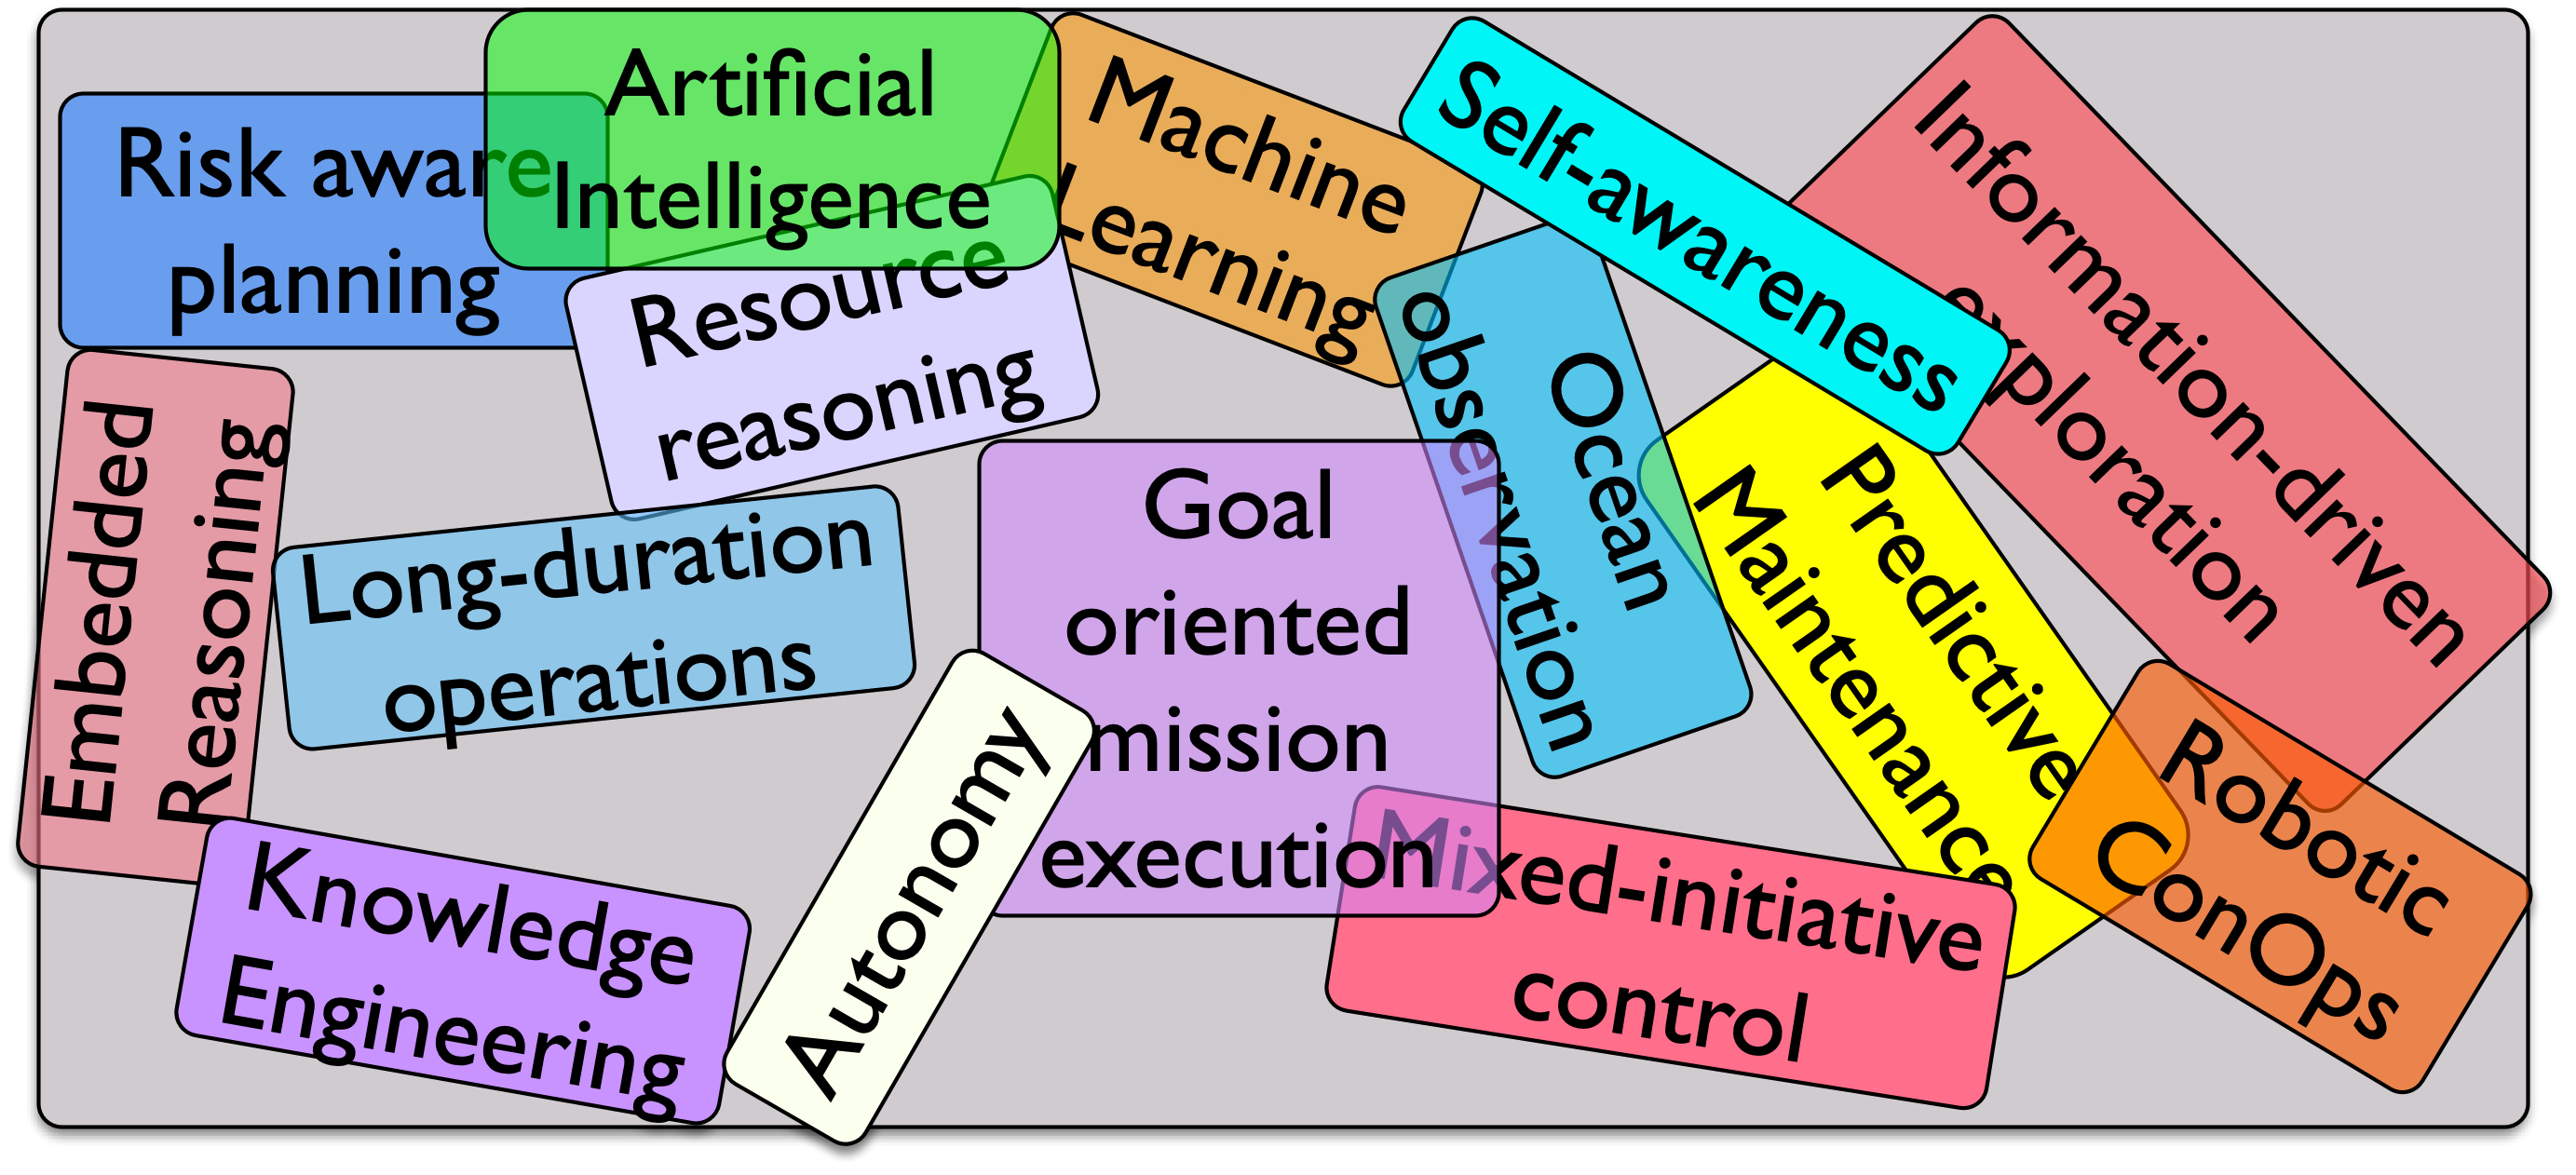
\includegraphics[scale=0.06]{fig/word-bag.jpg}
  \caption{Autonomous systems' use is across a range of domains and
    subject matter many of which are cross-cutting within \orge.}
 \label{fig:topics}
\end{wrapfigure}

Autonomous systems started as niche experimental platforms confined to
structured laboratory environments. Recently, they have increasing
seen operational use in real-world environments relevant to both
military and civil environments. Such systems are being introduced
across multiple topic areas (Fig. \ref{fig:topics}) across aerial,
terrestrial, as well as maritime domains (Fig. \ref{fig:inverse}). To
these we include the increasingly contested space domain, where
low-cost (in the millions of \$'s) small satellites are playing
significant roles in remote sensing and intelligence gathering.

\begin{wrapfigure}{!h}{3.2in}  
  \centering 
  \includegraphics[scale=0.05]{fig/inverse-pyramid.jpg} 
  \caption{A visualization of autonomous systems and their tools for
    exploration of our natural environment.}
  \label{fig:inverse}
\end{wrapfigure}

Autonomous platforms have been operating in multiple aerial domains
across the world for sometime; they are increasingly operating in the
Persian Gulf, the Black Sea, the Caribbean and the South China Sea to
name a few. Land based autonomous systems such as the Robotic Combat
Vehicle are planned to be inducted; \noae's use of manned airplanes
going thru Category 4 \& 5 hurricanes for data collection have given
way to the successful use of unmanned surface vehicles.

The primary \emph{modus-operandi} of such systems for now has been via
mixed-initiative (i.e. human-in-the-loop) control. This has allowed
placing the human well outside harms way, while also providing an
extension of the human senses. The technology roadmap of such systems
however, calls for 'dialing up' the autonomy in ways that embedded
machine intelligence (at the core of AI) can make decisions, drive
towards goal achievement and recover from failures, enabling
robustness and consistency in mission operations. Whether they augment
the warfighter, or completely replace them is likely to depend on a
range of issues spanning technology readiness to policy implications
of such self-aware fighting machines. But little thought has been
given within and outside \org to the implication of such robotic
warfighting, that we believe needs to be filled \emph{urgently}.

\pagebreak

The military space is not the only domain where autonomous systems are
(and likely to) have a lasting impact:

\subsubsection{Energy \& Environment}
\begin{itemize}

\item The Climate Change requires careful, systematic and
  \emph{at-scale} measurement collection and \emph{in-situ}. 70\% of
  the planet is water and many locations are hard to reach and/or
  hazardous to operate in. Autonomous systems can go where humans
  often cannot.

\item Ditto to the changing atmosphere and the warming it has led to
  over the poles, key areas of climate regulation.

\item Climatic impacts to weather resulting in adverse conditions have
  led to a range of adverse events including floods (flash and
  otherwise), tornadoes, hurricanes, and structural failures of man-made
  environments. 

\item The oceans have been to-date, a reliable carbon sink; yet our
  understanding of processes and how they're impacted with the
  increasing acidity as a result, has been narrowly focused on corals
  and their bleaching. More exploration (and over vast regions of
  uncharted waters) is needed to understand how the vastness of the
  seas and the life within is changing. This is not only tied to
  food-security of a range of developing coastal nations, but also its
  second-order effects related to shipping security (ref: Somalia,
  Nigeria and the Gulf of Guinea, Yemen).

\end{itemize}

\subsubsection{Healthcare \& Ageing}
\begin{itemize}
\item Japan and other low-birth rate nations are increasingly relying
  not on immigration, but on robots for elder care and observation. 

\end{itemize}

\subsubsection{Homeland Security and Public Safety}
\begin{itemize}

\item Police and security forces have come to embrace such
  technologies without due regard to implications of their use and the
  data they gather; this will only get worse.

\end{itemize}

Our longer term ambition is to establish a single 'go to' entity
within \org which will span across various divisions, including DPS,
SEW, NDRI, HSRD and the FFRDC's. This entity could be a 'center' which
can then be used as a focal point not just for cross-cutting work in
autonomous systems, but also for channelling funding including from
philanthropies and non-DoD sponsors.

\end{document}